
\section{Introduction}

\begin{frame}[fragile]
  \frametitle{Linguistic Approach}
  \vspace{-5mm}
  
  \begin{block}{}
    git \textipa{/gIt/}\\
    \textit{v Appalachian \& southern US}\\
    \hspace{1cm} variant of \emph{get}\\
    \textit{n Brit slang pejorative}\\
    \hspace{1cm} foolish or worthless person
  \end{block}
  \bigskip
  \pause

  \small
\begin{verbatim}
GIT(1)                   Git Manual                   GIT(1)

NAME
       git - the stupid content tracker

SYNOPSIS
       git [--version] [--help] [-c <name>=<value>]
           [--exec-path[=<path>]] [--html-path] [--man-path]
           ...
\end{verbatim}

\end{frame}


\begin{frame}
  \frametitle{Git, the DVCS}

  \begin{itemize}
  \item 
    Developed in 2005 to manage the Linux source code
    \begin{quote}
      I'm an egotistical bastard, and I name all my projects after
      myself. First ``Linux'', now ``git'' -- Linus Torvalds
    \end{quote}
  \item Slated to overtake \emph{Subversion} as the most popular VCS
    this year.
  \item \textbf{D}istributed -- there is no central server
  \item \textbf{V}ersion \textbf{C}ontrol \textbf{S}ystem -- manage
    changes to documents
  \item Git is free and open: \url{http://git-scm.com}
  \item Official \texttt{git} implementation: command-line program
  \item Various graphical user interfaces; I like \texttt{git-cola}
  \item Various websites offer git hosting (Github, Bitbucket,
    Mathematical Institute \url{https://git.maths.ox.ac.uk})
  \end{itemize}

\end{frame}



\begin{frame}
  \frametitle{Demo}
  
  Introduce the following commands:
  \begin{itemize}
  \item 
    Copy repository from github:\\
    \cmd{git clone}
    \\\hfill
    \cmd{https://github.com/vbraun/talk-git-sage-workflow.git}
  \item View history:\\
    \cmd{git log}
  \item Show current branch:\\
    \cmd{git branch}
  \item Switching between branches:\\
    \cmd{git checkout master}\\\cmd{git checkout my\_branch}
  \end{itemize}
\end{frame}


\begin{frame}
  \frametitle{The Git Directed Acyclic Graph}

  Whenever you run \cmd{git commit}, a snapshot of the current
  state\footnote{Of the \emph{staging} directory tree, see next
    slide.} is added to the repository.
  \begin{itemize}
  \item Only forward: you can add commits, but never remove them.
  \item But: you can abandon them.
  \item Most of the time, commits one (direct) parent commit and one
    child commit.
  \item Multiple parents: \emph{Merge} commit
  \item Number of children can change in the future...
  \end{itemize}
\end{frame}


{
  \usebackgroundtemplate{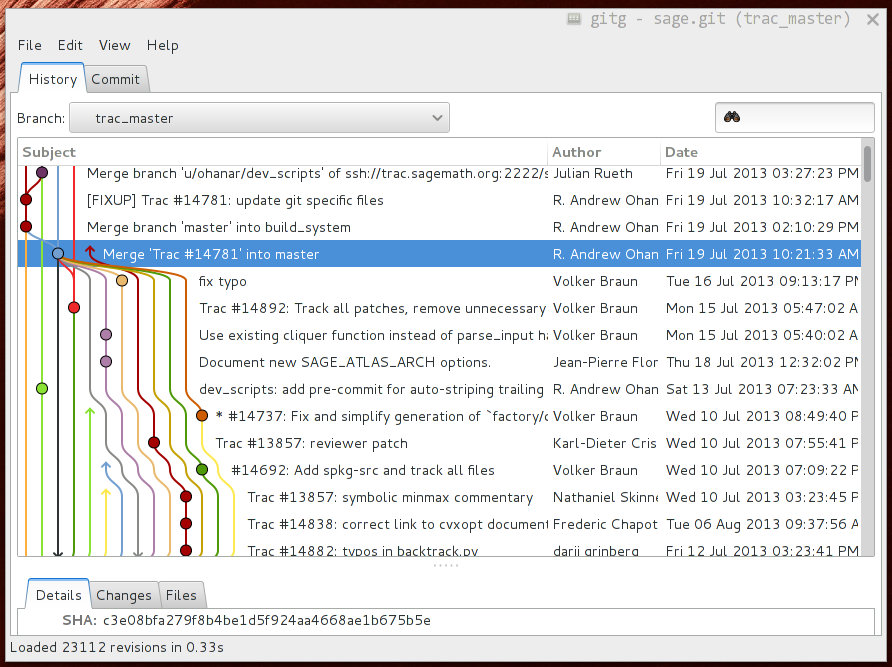
\includegraphics[width=\paperwidth]{images/gitg_screenshot}}
  \begin{frame}[plain]
    % 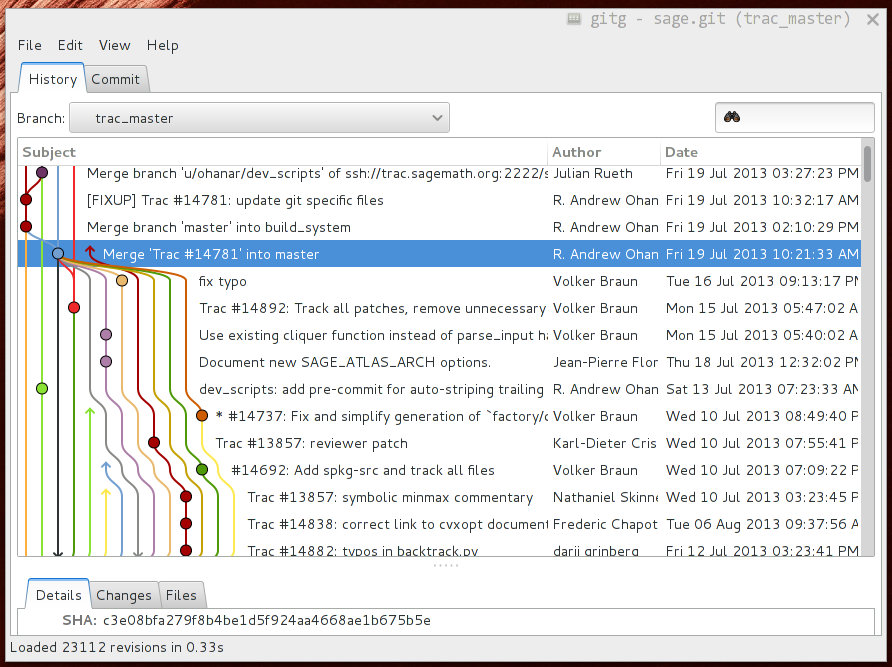
\includegraphics{images/gitg_screenshot}
  \end{frame}
}


\begin{frame}
  \frametitle{The Staging Area}

  Three places to store files:
  \begin{itemize}
  \item The git database (the \texttt{.git} directory)
  \item Staging area
  \item The working directory: all files outside of \texttt{.git} 
  \end{itemize}

  \begin{block}{Staging area}
    The staging area are the files that will be committed by
    \texttt{git commit}
    \begin{itemize}
    \item Show staging: \cmd{git status}
    \item Add to staging: \cmd{git add <filename>}
    \item Remove from staging: \cmd{git reset HEAD <filename>}
    \end{itemize}
  \end{block}
\end{frame}




\begin{frame}
  \frametitle{Committing Changes}

  The changes are 
\end{frame}




%%% Local Variables:
%%% TeX-master: "talk"
%%% eval: (TeX-PDF-mode 1)
%%% End:
